\documentclass[10pt]{article}
\usepackage[T1]{fontenc}
\usepackage[utf8]{inputenc}
\usepackage[italian]{babel}
\usepackage{multicol}
\usepackage[a4paper, total={18cm, 25cm}]{geometry}
\usepackage{amsfonts}
\usepackage{lmodern}
\usepackage{graphicx}
\graphicspath{ {./img/} }

\begin{document}
{\fontfamily{lmss}\selectfont
\title{Università di Pisa\\Reti di Calcolatori e Laboratorio\\Word Quizzle -- Relazione}
\author{Federico Matteoni\\Matricola 530257}
\date{ }
\renewcommand*\contentsname{Indice}

\maketitle
\section{Introduzione}
\paragraph{Funzionalità} Il progetto richiedeva lo sviluppo di \textbf{WordQuizzle}: un sistema di sfide di traduzione italiano--inglese tra gli utenti registrati al servizio.\\
Era richiesta la possibilità, per gli utenti registrati, di poter sfidare gli utenti appartenenti alla propria rete sociale di amicizie. Le sfide consistevano nella traduzione, nel minor tempo possibile, di una serie di parole italiane proposte dal servizio.
\paragraph{Architettura} Si richiedeva che l'applicazione fosse implementata secondo un'architettura client--server, con i componenti che comunicano \texttt{TCP}, \texttt{UDP} e tramite il meccanismo \texttt{RMI}. Inoltre si richiedeva, per il server, la persistenza delle informazioni degli utenti su un file \texttt{JSON}, e la richiesta delle traduzioni delle parole scelte ad un servizio esterno tramite richieste \texttt{HTTP GET}.\\
L'interazione con l'utente poteva avvenire tramite una \texttt{CLI} oppure, opzionalmente, una \texttt{GUI}. Per sperimentazione e sfida personale ho scelto la seconda.
\section{Overview del sistema}
Il sistema è suddiviso in due parti principali: \textbf{client} e \textbf{server}. Tramite il client è possibile interagire col servizio WordQuizzle, che viene offerto dal server.\\
L'\textbf{interfaccia del server} offre varie \textbf{informazioni sullo stato attuale del servizio}, dagli utenti alla porta usata. Può essere usata per verificare il corretto funzionamento del sistema e monitorare le sfide in corso.\\
L'\textbf{interfaccia del client} è usata per l'\textbf{interazione vera e propria} col servizio: da essa si possono lanciare le sfide, richiedere le informazioni al server e consultare la propria lista amici e lo stato del proprio profilo utente.
\subsection{Istruzioni per la compilazione}
Il progetto è stato sviluppato mediante l'IDE IntelliJ IDEA, utilizzando come libreria esterne la libreria \textbf{GSON}\\(\texttt{com.google.code.gson}) in versione 2.8.5. Sarà necessario specificare tale libreria nel build path per poter compilare il progetto.
\subsection{Istruzioni per l'installazione e l'avvio}
\paragraph{Server} Il server, eseguito dall'archivio \texttt{WordQuizzleServer.jar}, \textbf{deve essere eseguito in una directory contenente un file chiamato "dizionario"}, contenente il dizionario da cui selezionare le parole per la sfida. Il dizionario contiene \texttt{N} parole italiane, una per riga. Un dizionario di esempio con 100 parole è incluso.\\
Per avviare il server, è sufficiente eseguirlo con il comando \texttt{java -jar WordQuizzleServer.jar <porta>}, passando il numero di porta su cui stabilire le connessioni con il parametro \texttt{<porta>}.
\paragraph{Client} Il client viene eseguito a partire dall'archivio \texttt{WordQuizzleClient.jar} tramite il comando\\\texttt{java -jar WordQuizzleClient.jar <porta>}, specificando la porta del server a cui collegarsi tramite il parametro \texttt{<porta>}.
\pagebreak
\subsection{Server}
\begin{center}
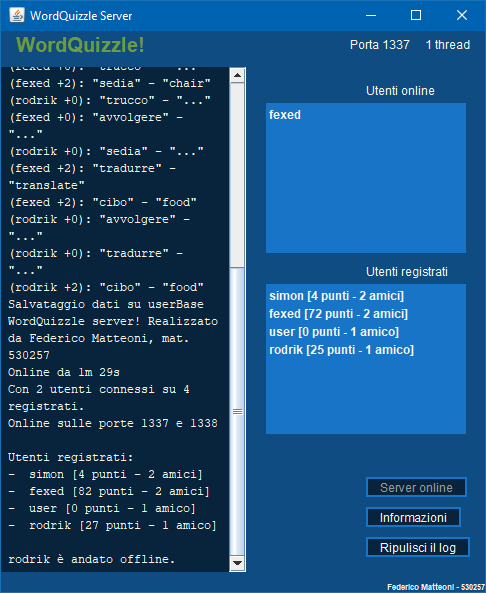
\includegraphics[scale=0.75]{server.png}
\end{center}
\paragraph{Interfaccia} L'interfaccia del server è strutturata in modo da fornire a colpo d'occhio informazioni utili quali: utenti online e registrati, eventi recenti del servizio come sfide, connessioni e disconnessioni.\\
L'interfaccia cerca di essere il più chiara e intuitiva possibile: sulla sinistra si trova il log del servizio, mentre sulla destra sono elencati gli utenti online, quelli registrati e i comandi per avviare il server, stampare delle informazioni utili sul log o ripulirlo. In alto sono indicati il numero di porta su cui il server ascolta le connessioni in arrivo e il numero di thread attualmente eseguiti dal server.\\
La scritta "WordQuizzle" in alto a sinistra viene colorata di rosso o di verde a seconda dello stato in cui si trova il server, rispettivamente offline od online.
\paragraph{Funzionalità} Il server si avvia automaticamente al lancio dell'eseguibile, ascoltando sul numero di porta specificato. Può essere chiuso come una qualsiasi applicazione dalla \texttt{X} in alto a destra sulla barra del titolo della finestra. In caso di errori ed eccezioni, il server stamperà i messaggi di errore sullo standard output (solitamente, la console da dove è stato lanciato) per poter verificare il messaggio dell'errore che si è verificato.\\
Quanto al servizio WordQuizzle, è possibile fare doppio click su un utente registrato per poter verificare le sue informazioni quali nome utente, password e punteggio, oltre alle amicizie nel dettaglio.
\begin{center}
Le informazioni di un utente\\
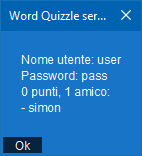
\includegraphics[scale=1]{infouser.png}
\end{center}
\pagebreak
\subsection{Client}
\begin{center}
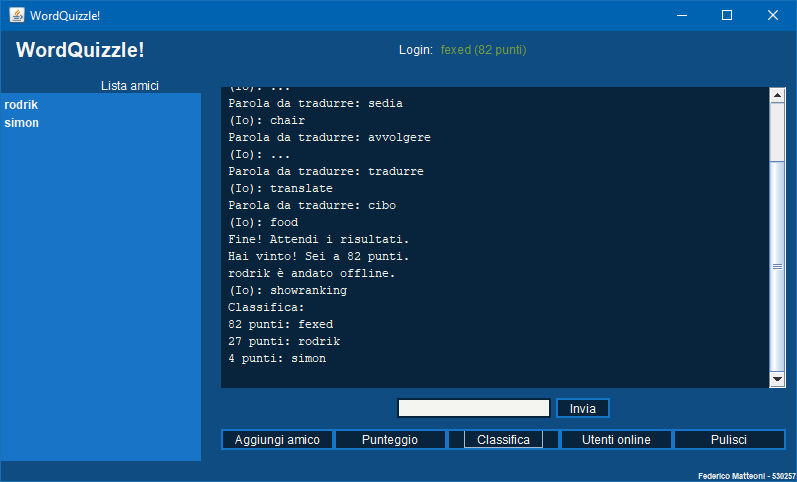
\includegraphics[scale=0.75]{client.png}
\end{center}
\paragraph{Interfaccia} L'interfaccia dell'utente è pensata per essere facilmente fruibile in modo da ottenere le informazioni necessarie dal server o sfidare rapidamente un utente della propria lista amici. La finestra presenta al centro il log dei messaggi spediti e ricevuti dal server, mentre sulla sinistra c'è la lista amici dell'utente connesso. Le informazioni dell'utente sono visibili in alto, con punteggio e nome utente colorato di verde o rosso a seconda se il client è, rispettivamente, connesso o meno.\\
In basso si trova la barra di testo in cui inserire i comandi o, durante una sfida, le traduzioni proposte. Il pulsante "\texttt{Invia}" è selezionabile anche con il tasto \texttt{Invio} della tastiera, per permettere allo sfidante di rispondere il più velocemente possibile durante la sfida di traduzione. I pulsanti inferiori mandano dei messaggi che il server interpreta come richiesta di informazioni.\\
Il pulsante "\texttt{Aggiungi amico}" apre una finestra di dialogo che richiede il nickname dell'utente da aggiungere.\\
La finestra di \textbf{login} si apre automaticamente all'avvio del client, mentre in caso di caduta della connessione e client offline apparirà un pulsante "\texttt{Login}" a destra del punteggio, per poter reinstaurare la connessione.
\paragraph{Funzionalità} Per poter \textbf{sfidare un amico} è sufficiente fare doppio click sul nome utente dell'amico che si vuole sfidare. Il sistema gestirà la richiesta e la risposta: una finestra di dialogo apparirà sul client dell'amico che si vuole sfidare e attenderà una risposta per 10s. In caso di risposta affermativa, la sfida partirà per entrambi gli utenti.\\
L'aggiunta di un amico, la richiesta di punteggio, classifica e utenti online sono tutte funzionalità richiedibili tramite gli appositi pulsanti nella parte inferiore dell'interfaccia.\\
Eventuali errori che richiedono attenzione sono visualizzati come finestra di dialogo contenente il messaggio d'errore.
\begin{multicols}{2}
\begin{center}
La finestra di login\\
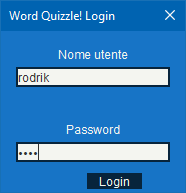
\includegraphics[scale=1]{login.png}
\end{center}
\begin{center}
La richiesta di sfida\\

\includegraphics[scale=1]{sfida.png}
\end{center}
\end{multicols}
\pagebreak
\section{Funzionalità}
Dettaglio delle varie funzionalità del servizio che sono state richieste e delle scelte in sede di implementazione.
\subsection{Registrazione}
La fase di \textbf{registrazione} è stata implementata sfruttando la tecnologia \textbf{RMI} come richiesto.\\Il \textbf{server} pubblica, sulla porta successiva a quella indicata come parametro, il riferimento alla propria interfaccia di registrazione con chiave "\texttt{WordQuizzle\_530257}" per evitare possibili conflitti.\\
Il \textbf{client} esegue la procedura di registrazione in fase di login: se l'utente non esiste allora verrà registrato con il nome utente e la password appena inseriti. La fase di registrazione darà quindi errore in caso di nome utente già registrato oppure in caso di password vuota, oltre al caso in cui si verificano eventuali errori di comunicazione.

\subsection{Login}
La fase di \textbf{login} è eseguita quando l'utente ha inserito nome utente e password nella finestra di dialogo apposita e confermato l'inserimento. Il \textbf{client} spedisce via TCP un messaggio del tipo \texttt{login:nomeutente password}.\\
Il \textbf{server} verifica la correttezza dei dati e restituisce il risultato, con un messaggio del tipo \texttt{answer:esito}.
\paragraph{Errore} In caso di errore, come password vuota o sbagliata o utente già collegato, il server ritorna un codice di errore apposito e il client mostrerà l'errore in una finestra di dialogo, per poi richiedere nuovamente i dati di login.
\paragraph{Successo} In caso di login eseguito con successo, il server lancerà un \textbf{thread gestore} dedicato al client e alla sua connessione. Il server mantiene in memoria un riferimento al gestore legato al nome utente che gestisce: questo è utile per mantenere la lista degli utenti connessi e poter spedire le richieste di sfida.\\
Subito dopo il server spedisce al client un \texttt{JSON} con le informazioni dell'utente connesso: punteggio e lista amici. Questo per consentire al client di aggiornare la propria interfaccia di conseguenza.\\
Il client comunicherà al server la propria porta UDP per ricevere le richieste di sfida con un messaggio del tipo\\\texttt{challengePort:porta}.

\subsection{Logout}
Il logout viene eseguito alla chiusura della finestra del client. Il client chiuderà il socket di comunicazione, terminando il thread gestore associato sul server, il quale si preoccuperà di aggiornare il conteggio dei thread attivi e la lista degli utenti connessi.

\subsection{Aggiunta di un amico}
La fase di aggiunta di un utente alla propria lista amici si avvia cliccando sul relativo pulsante nell'interfaccia del client. Esso aprirà una finestra di dialogo richiedente il nome dell'utente da aggiungere.\\
In caso di conferma, il client spedirà al server un messaggio del tipo \texttt{addfriend:nomeutente} e attenderà il messaggio di risposta dal server, che può essere \texttt{anser:OKFREN} oppure \texttt{answer:ERR messaggio}.
\paragraph{Errore} In caso di errore verrà semplicemente stampato il messaggio d'errore ricevuto sul log del client, consentendo all'utente di verificare cos'è andato storto. L'errore in questa fase può avvenire per aver tentato di aggiungere come amico un utente inesistente, già nella lista amici o sé stessi.
\paragraph{Successo} In caso di successo, il server si occuperà di aggiungere gli utenti come amici, aggiornando la lista amici di entrambi. Il client dopodiché richiederà la lista amici al server così da mostrare all'utente l'effettiva aggiunta del nuovo amico e poter aggiornare l'interfaccia.

\subsection{Richiesta della lista amici}
Alla pressione del relativo pulsante sull'interfaccia del client, verrà spedito un messaggio del tipo \texttt{showfriendlist} al server. Esso risponderà con un messaggio del tipo \texttt{friendlist:JSON}, con il JSON rappresentante la struttura dati della lista amici (\texttt{WQUtente[]}). Per i dettagli delle classi si veda la sezione apposita.\\
Il client stamperà sul log la lista degli amici e aggiornerà l'interfaccia con la lista amici appena ricevuta.

\subsection{Richiesta della lista degli utenti online}
Analogamente, alla pressione del pulsante relativo il client invia \texttt{showonlinelist} al server, che risponderà con \texttt{onlinelist:JSON}. Il JSON rappresenta la lista degli utenti online (\texttt{ArrayList<WQUtente>}) che il client visualizzerà nel log.

\subsection{Richiesta del punteggio utente}
Il client spedisce \texttt{showpoints} al server, che risponde con \texttt{userpoints:punti}. Il punteggio ricevuto è visualizzato sul log e usato per aggiornare l'interfaccia del client.

\subsection{Richiesta della classifica}
La classifica è richiesta con un messaggio del tipo \texttt{showonlinelist}. Il server risponderà con la classifica come JSON (\texttt{ArrayList<WQUtente>}) in un messaggio del tipo \texttt{ranking:JSON}.

\subsection{Sfida}
La sfida è implementata, come richiesto, spedendo la richiesta (\texttt{challengeRequest:sfidante}) tramite UDP allo sfidante. La porta UDP su cui spedire la richiesta è comunicata dal client a seguito del login.\\
La sfida deve essere accettata entro (\textbf{T1}) 10 secondi. Se la sfida viene rifiutata (\texttt{challengeResponse:NO}, sia per timeout che per rifiuto esplicito), il server lo comunicherà al client che l'ha richiesta, il quale visualizzerà sul log il messaggio "\texttt{La sfida è stata rifiutata.}".
\paragraph{Sfida accettata} Se la sfida viene accettata (\texttt{challengeResponse:OK}), il server comunica ad entrambi i client di prepararsi con un messaggio del tipo \texttt{challengeRound:1}.
\subparagraph{Parole} Il server, quindi, seleziona (\textbf{K}) 6 parole casuali dal dizionario, che contiene (\textbf{N}) 100 parole, e richiede le traduzioni al servizio esterno \texttt{mymemory.translated.net} tramite una serie di richieste \texttt{HTTP GET}. Per ogni parola italiana viene memorizzata la lista delle traduzioni fornite dal servizio. Le parole vengono ottenute eseguendo un parsing del \texttt{JSON} restituito, con tutte lettere minuscole e ripulendole da caratteri non alfabetici.
\subparagraph{Sfida} Non appena sono state ottenute tutte le traduzioni, il server lancia un \textbf{thread arbitro} che gestisce la sfida. Il thread si occupa di fornire ai thread gestori dei due utenti le parole da tradurre e le traduzioni, e attende che entrambi gli sfidanti abbiano finito la sfida.\\
Ogni thread gestore spedirà la parola da tradurre in un messaggio \texttt{challengeRound:parola} e attende un messaggio di risposta del tipo \texttt{challengeAnswer:parola}. Il client concede all'utente 5s per rispondere: la sfida può durare quindi al massimo K$\cdot$5s cioè (\textbf{T2}) 30 secondi. Se il timer scade, il client risponde automaticamente con \texttt{challengeAnswer:-1}, altrimenti risponde con la parola inserita dall'utente.\\
Il thread gestore verifica le traduzioni, assegnando (\textbf{X}) 2 punti per traduzione corretta e togliendo (\textbf{Y}) 1 punto per ogni risposta sbagliata. In caso di risposta non data, non si assegnano punti.
\subparagraph{Fine} Non appena entrambi gli utenti hanno concluso la sfida, il thread arbitro si occupa di verificare il vincitore comparando i punteggi ottenuti. L'utente vincitore ottiene (\textbf{Z}) 5 punti bonus.\\
L'arbitro comunica il risultato agli sfidanti, mandando un messaggio del tipo \texttt{answer:challengeWin punti} al vincitore e \texttt{answer:challengeLose punti} al perdente, indicando anche il nuovo punteggio utente a ciascuno. In caso di pareggio, entrambi gli sfidanti riceveranno \texttt{anser:challenge punti}.\\
Dopodiché, vengono salvati i dati del server e la sfida è conclusa.
\pagebreak
\section{Struttura del codice}
Dettaglio delle classi, della loro organizzazione e delle loro funzionalità in generale.
\begin{list}{}{Classi comuni ai due componenti}
	\item \textbf{WQGUI}: include colori, tema e codice di inizializzazione dei componenti comuni alle \texttt{GUI}.
	\item \textbf{WQInterface}: interfaccia per la registrazione tramite \texttt{RMI}.
	\item \textbf{WQUtente}: dati del singolo utente, come nome utente, password, punteggio e lista amici.
\end{list}
\begin{list}{}{\textbf{Server}}
	\item \textbf{Logica}
	\item \textbf{WQServer}: codice principale del server, che implementa tutte le funzionalità richieste, tra cui la registrazione, login, sfida e strutture dati principali.
	\item \textbf{WQHandler}: \textbf{thread gestore} della connessione con il singolo client, che si occupa di spedire e ricevere i messaggi sia su \texttt{TCP} che le richieste e risposte di sfida su \texttt{UDP}. Si occupa anche della parte centrale della sfida, cioè invio delle parole e ricezione delle risposte con calcolo del punteggio.
	\item \textbf{WQRefree}: \textbf{thread arbitro} della sfida. Si occupa di lanciare la parte centrale della sfida e attendere la fine di entrambi gli sfidanti, dopodiché decreta il vincitore e assegna il punteggio definitivo.
	\item \textbf{Interfaccia}
	\item \textbf{WQServerController}: permette la comunicazione tra server e \texttt{GUI}.
	\item \textbf{WQServerGUIInterface}: interfaccia della \texttt{GUI} del server, per poter aggiornare i vari componenti all'accadere dei vari eventi.
	\item \textbf{WQServerGUI}: codice di creazione, comportamento e visualizzazione della \texttt{GUI} del server. Inoltre è la classe principale contenente il \textbf{main} del server.
\end{list}
\begin{list}{}{\textbf{Client}}
	\item \textbf{Logica}
	\item \textbf{WQClient}: codice principale del client, che implementa le funzionalità di login, registrazione e comunicazione principale del client.
	\item \textbf{WQClientReceiver}: \textbf{thread} di ascolto del client per ricevere i messaggi \texttt{TCP} del socket provenienti dal server.
	\item \textbf{WQClientDatagramReceiver}: \textbf{thread} di ascolto del client per ricevere i messaggi \texttt{UDP} provenienti dal server. Gestisce tutte le richieste di sfida ricevute, ma consente di rispondere ad esse solamente se non si è già in una sfida.
	\item \textbf{WQClientTimerTask}: \texttt{TimerTask} del client per il tempo di risposta durante la sfida. Viene eseguito allo scadere del timer di 10 secondi, che parte alla ricezione di una parola da tradurre.
	\item \textbf{Interfaccia}
	\item \textbf{WQClientController}: permette la comunicazione tra client e \texttt{GUI}.
	\item \textbf{WQClientGUIInterface}: interfaccia della \texttt{GUI} del client, per poter aggiornare i vari componenti all'accadere dei vari eventi.
	\item \textbf{WQClientGUI}: codice di creazione, comportamento e visualizzazione della \texttt{GUI} del client. Inoltre è la classe principale contenente il \textbf{main} del client.
\end{list}
\section{Librerie utilizzate}
Per la serializzazione e la trasformazione dei dati di WordQuizzle in e da \texttt{JSON} è stata utilizzata la libreria \textbf{GSON}, che permette facilmente di trasformare oggetti Java in \texttt{JSON} e oggetti \texttt{JSON} in oggetti Java conoscendone il tipo originale.\\
Per il parsing dei dati \texttt{JSON} ricevuti dal servizio esterno è stata usata la stessa libreria.\\
Tale libreria è inclusa negli archivi \texttt{JAR} forniti.
\pagebreak
\section{Thread e Strutture dati}
\subsection{Client}
Il client lavora su 3 \textbf{thread} distinti:
\begin{list}{-}{}
	\item Il \textbf{thread GUI}, che aggiorna e smista gli eventi dell'interfaccia grafica.
	\item Il \textbf{thread principale}, che riceve i messaggi \texttt{TCP} dal server e li elabora, gestendo login, richieste al server e lo scambio di messaggi durante la sfida
	\item Il \textbf{thread UDP}, che riceve i messaggi \texttt{UDP} dal server e li elabora. Permette di accettare solamente una sfida alla volta, rifiutando automaticamente se il client è già nel mezzo di una sfida.
\end{list}
Come \textbf{strutture dati}, il client mantiene i dati sulla comunicazione (socket e porta) e i dati dell'utente, come nome utente, punteggio e amici.
\subsection{Server}
Il server è così strutturato:
\begin{list}{-}{}
	\item \textbf{Thread principale}, che ascolta le connessioni dei nuovi client e smista le connessioni in entrata assegnandole ad un thread gestore
	\item \textbf{Thread gestori}, uno per client. Gestiscono la comunicazione con quel client e lo scambio di messaggi. Si occupa anche di mandare le richieste di sfida via UDP.\\
	L'aggiornamento e la consultazione delle strutture dati degli utenti collegati e registrati è eseguito da un metodo \texttt{synchronized} per garantire la sincronizzazione tra i vari gestori.
	\item \textbf{Thread arbitri}, uno per sfida. Gestiscono la sfida, attendendo la conclusione di ogni utente e decretando l'esito, comunicandolo.
\end{list}
Le \textbf{strutture dati} più importanti del server sono le seguenti:
\begin{list}{-}{}
	\item \textbf{\texttt{userBase}}: mappa ad ogni nome utente la struttura dati relativa a quell'utente, cioè password, punteggio e lista amici.
	\item \textbf{\texttt{loggedIn}}: mappa ad ogni nome utente il thread gestore che lo sta gestendo. Grazie a questa lista è possibile verificare se un utente è connesso, quanti utenti connessi ci sono e spedire un messaggio ad un utente specifico.
	\item Ogni server mantiene lo username dell'utente che sta gestendo e i dati della comunicazione (porte e socket)
\end{list}
\section{Possibili estensioni}
Il sistema è potenzialmente estendibile sotto qualche aspetto. Ad esempio la comunicazione implementata è facilmente estendibile a sistema di chat interno alla rete sociale di un dato utente: questo è possibili apportando alcune modifiche all'elaborazione che il server fa di ogni messaggio, in modo che smisti tale messaggio al gestore di ogni utente amico attualmente online.\\
Il dizionario mantenuto dal server può essere aggiornato o esteso da qualche servizio esterno, mediante un meccanismo simile a come si ottengono le traduzioni.\\
Inoltre, nell'implementazione è stata volutamente tralasciata la crittografia delle password degli utenti, poiché ritenuta non interessante ai fini delle richieste e potenzialmente di difficile implementazione.\\
Queste e altri possibili estensioni sono state tralasciate in favore di un codice più contenuto e più concentrato sulle funzionalità richieste.
}
\end{document}